\section{Microservices}
    We did a server and ran it with only one executable file, one application deployed even if it's running on four cores. It is called a monolith.
    \begin{tcolorbox}[vert]
        A \important{monolith} is a single application that contains all the functionality. All functions are part of the same program and run in the same address spaces.
    \end{tcolorbox}
    Real-world monoliths are complex and contain several functions, it suffer from synchronization overheads among threads, it doesn't scale well. Overhead limit monoliths from fully utilizing all the cores and there is synchronization limits performance beyond a few cores. In resume, there is a lot of part that are dependent and should be synchronized.
    \begin{tcolorbox}[rouge]
        A solution to use cores effectively is to run multiple monolith copies. Each instance behaves as an independent server, threads among different instances shouldn't synchronize with each other. Also, each instance runs on a smaller number of cores and scales well.
    \end{tcolorbox}
    \begin{center}
        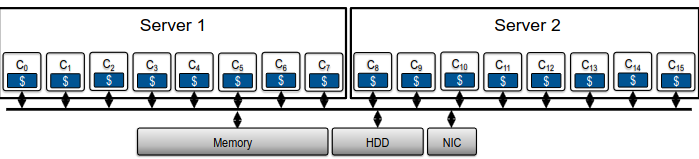
\includegraphics[width=12cm]{images/61.png}
    \end{center}
    But monoliths use other resources too:
    \begin{itemize}[left=10pt, label=\textbullet]
        \item Memory capacity: each monolith can take a big chunk of server's memory. 

            If each instance of a server can consume a large amount of memory (e.g. 60\% of the system's total memory capacity), then you can't run many instances together on the same server.
        \item Memory bandwidth: Analytic workloads scale well but use a lot of memory bandwidth. 
        \item NIC bandwidth: performance may be limited based on availability of NICs. 
        \item Accelerators: GPUs in a server may require CPU cores for coordination.
    \end{itemize}
    \begin{tcolorbox}[violet]
        A monolith does not provide strong isolation between functions: for example, a third-party cryptographic function like \texttt{sha} and an internal function like \texttt{save\_file} run inside the same process and cannot be executed separately, since they share the same runtime and resources, which tightly couples them at runtime.
    \end{tcolorbox}
    Now that we saw every disadvantages of monolith, how can we improve this?\\

    In our web server, we can maybe group our functions based on the type of task they perform. We clearly have two distinct types of tasks:
    \begin{enumerate}[left=10pt]
        \item Save and serve files (\texttt{save\_file} and \texttt{get\_line})
        \item Perform hash computations (\texttt{sha})
    \end{enumerate}
    \begin{center}
        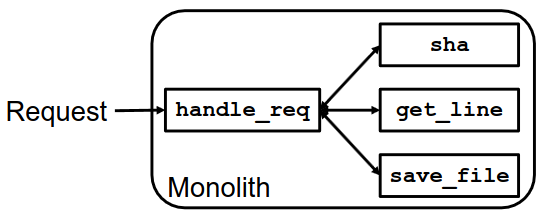
\includegraphics[width=7cm]{images/63.png}
    \end{center}
    These two tasks are independent, they can be separated logically and physically !
    \begin{tcolorbox}[vert]
        Groups of functions can be treated as separate ``services'' based on functionality and needs. Services have separate codebases, address spaces, etc\ldots This is called a \important{microservice architecture}: a set of small (micro), independent and self-contained services.
    \end{tcolorbox}
    A service executes a single task type in isolation, each service has its own address to receive requests. Each service has also its own copy of \texttt{handle\_request}, processes incoming requests and chooses which function to execute.

    \begin{center}
    \begin{tabular}{c|ccc}
        \textbf{Monolith} & \textbf{Microservices}  \\
        \hline  \\
        
        One big program containing all functions & Functions are grouped into small programs (services)  \\
         \\
        \hline \\
        
        All functions run in 

        the same address space & Each service runs in its own address space  \\
        
         \\
        \hline \\
        
        Functions call other functions and use & Functions in various services can also ``call'' each other and \\
        shared memory to communicate & communicate using messages (in detail later) \\
         \\
        \hline
    \end{tabular}
    \end{center}
    \begin{tcolorbox}[gris]
           Services have various system requirements: e.g. \texttt{file.py} (to handle file) will use more memory but \texttt{hash.py} (to crypt) will use more compute. \\

       Services are not used uniformly: some services are more popular than others, they will handle more requests.\\

       With microservice each service can be scaled independently of the others: popular services can be scaled without scaling the other services and resources can be better allocated depending on each service's needs.
            
        
    \end{tcolorbox}
    Before, we saw that if our server use eight cores and 60\% of the system's total memory then we can only run one server. Now we can completely utilize all cores and memory:
    \begin{center}
        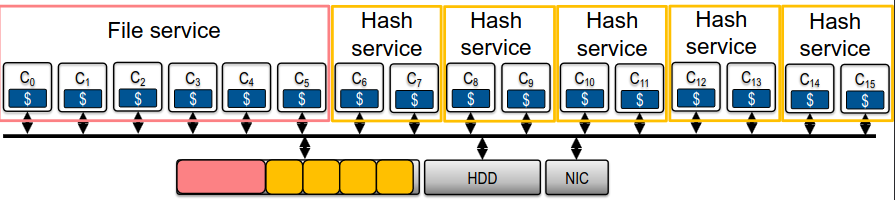
\includegraphics[width=13cm]{images/64.png}
    \end{center}
    \begin{tcolorbox}[rouge]
    Other's advantages are:
    \begin{itemize}[left=10pt, label=\textbullet]
        \item Services can be written independently of each other and we can choose the best programming language according to a service's needs.
        \item We can have cheaper plans: cloud providers offer servers with different price in function of resources that they have (e.g. memory).
        \item There is more fault tolerance: one service failing doesn't lead to the entire workload failing.
        \item It allows re-usability: services are isolated but can be accessed from any other service.
    \end{itemize}
    \end{tcolorbox}
    But there is also disadvantages! Services have to communicate between them by messages, it becomes critical as the number of services increases.
    \begin{remark}{Remark}
        Connectivity graph are important for scalability:\\
            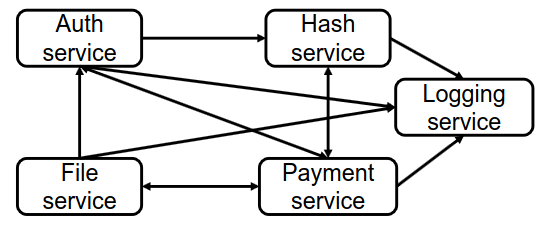
\includegraphics[width=6cm]{images/65.png}
    \end{remark}
    The communication protocol of microservices must be:
    \begin{itemize}[left=10pt, label=\textbullet]
        \item fast,
        \item fault-tolerant, 
        \item able to locate each service on the network, 
        \item able to pass input on the service and receive its output.
    \end{itemize}
    \subsection{RPC}
    Microservices communicate as if via function calls.
    \begin{tcolorbox}[vert]
        There is local calls that are calls by a function to another function within the same service. This is our conventional function call. We call this \important{local procedure call (LPC)}.
    \end{tcolorbox}
    \begin{tcolorbox}[vert]
        There is remote calls that are calls by a function to another function in a different service. This is new and used for microservices. We call this \important{remote procedure call (RPC)}.
    \end{tcolorbox}
    To first define our function, we use an interface definition language (IDL): this language will not run any code, it's a common format to describe functions across languages.\\

    \begin{tcolorbox}[violet]
    We first have just to define the interface of our function, not an implementation:
    \begin{codeCenter}
    \begin{Ccode}
service hash{
    rpc sha(Request) returns (StringValue) {}
}
    \end{Ccode}
    \end{codeCenter}
        The RPC library has implementation for various languages like C, Python, etc\ldots It will take in the interface definition code as input and will generate code in the language of all our services from one interface definition code.\\

    The code generated for the service that implements and serves a function is called the server stub. The server stub will just be an abstract function, the developer have to implements it.
    \begin{codeCenter}
    \begin{Ccode}
// generated by rpc library in C for the hash service
class HashService::service{
    // Abstract function, later implemented by developer
    virtual char * sha(Request req)= 0;
}
    \end{Ccode}
    \end{codeCenter}

    The code generated for the services that use a function is called the client stub. This is a concrete code that RPC will implement sending the request to the service that serves it.
    \begin{codeCenter}
    \begin{Ccode}
# generated by rpc library in Python for the file service
class HashService:
    def sha(req: Request)-> String:
        # RPC sending the request to hash service
        resp = sendReq(req)
        ...
    \end{Ccode}
    \end{codeCenter}
    \end{tcolorbox}
    In our server case, the \texttt{hash\_file} function is using \texttt{sha} function. So it will look like this:
    \begin{center}
        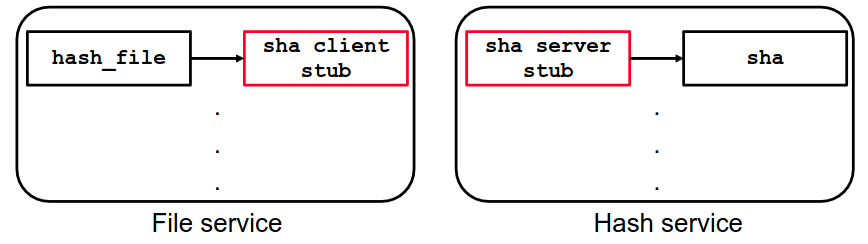
\includegraphics[width=9cm]{images/66.png}
    \end{center}
    We can't directly transfer data between stubs, because languages stores types in various formats in memory. So we have to do marshalling/unmarshalling.
    \begin{tcolorbox}[vert]
        \important{Marshalling} turn data from a memory representation into a representation that can be sent over the network. RPC unifies marshalling data for all services, once received RPC needs to be able to save it to memory again.
    \end{tcolorbox}
    \begin{tcolorbox}[vert]
        \important{Unmarshalling} turn data received from the network in an IDL representation into a memory representation of the receiving language.
    \end{tcolorbox}
    \begin{center}
        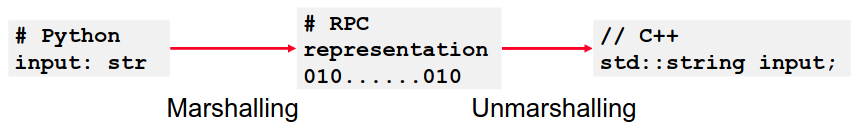
\includegraphics[width=11cm]{images/67.png}
    \end{center}
    \begin{tcolorbox}[gris]
        
    
    To call a function, for example \texttt{hash\_file} that calls \texttt{sha}, it works like this:
    \begin{enumerate}[left=10pt]
        \item \texttt{hash\_file} calls the client stub's \texttt{sha} function with its inputs. 
        \item Client stub's \texttt{sha} function takes the input and marshalls data from memory into a representation that can be sent over the network (RPC provide the send function to send marshalled data).
        \item Marshalled data is sent to hash service, RPC libraries include a built-in server that listens for RPC requests coming in from the network.
        \item Server stub's \texttt{sha} function takes the input and unmarshalls the data into variables that can be used by functions.
        \item It calls the functions \texttt{sha}.
        \item Server stub marshall the result and sends it back to the caller.
        \item Client stub unmarshalls the result and returns it to \texttt{hash\_file}. 
    \end{enumerate}
    All these steps are generated by RPC.
    \end{tcolorbox}
    \begin{center}
        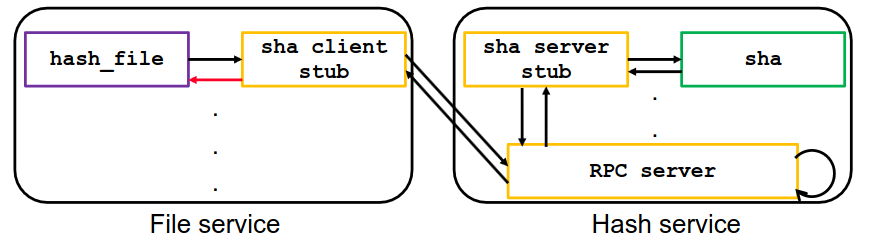
\includegraphics[width=9cm]{images/68.png}
    \end{center}
    \begin{codeCenter}
    \begin{Ccode}
# generated client stub by rpc library for file service
class HashService:
    sha(self, input):
        req = marshall(input)
        resp = send(req)
        return unmarshall(resp)
    \end{Ccode}
    \end{codeCenter}
    \subsubsection{gRPC}
    There is multiple RPC, we'll see for example gRPC that uses protocol buffers (protobuf) as IDL.
    \begin{center}
        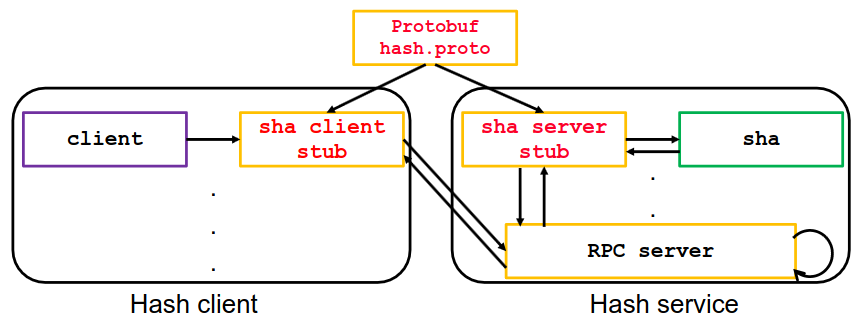
\includegraphics[width=9cm]{images/69.png}
    \end{center}
    The code of declaration of function would then look like this:
    \begin{codeCenter}
    \begin{Ccode}
// hash.proto
syntax = "proto3"; // Define protobuf syntax

message HashRequest {
    string input = 1; // One is the ordered attribute for serialization
}

message HashResult {
    string result = 1;
}

service Hash {
    rpc GetHash (HashRequest) returns (HashResult);
}
    \end{Ccode}
    \end{codeCenter}
    \begin{tcolorbox}[rouge]
        IDL's need to be compiled to be used, here protoc is the official protobuf compiler.
        \begin{codeCenter}
        \begin{Ccode}
pip install grpcio-tools // install compiler

python -m grpc_tools.protoc \ // starting it
        -I .               \ // IDL folder
        --pyi_out=.         \ // output destination
        --python_out=.      \ // output destination
        --grpc_python_out=. \ //  output destination
        hash.proto            //IDL file
        \end{Ccode}
        \end{codeCenter}
    \end{tcolorbox}
    Each .proto file will generate a \texttt{\_pb2.py} file that contains the definition of all inputs and outputs and implements marshalling and unmarshalling for inputs and outputs.\\
    
    It will also generate a \texttt{\_pb2\_grpc.py} file that contains the definition of the services: the abstract class to be implemented in the server and the stub class to be used as substitute by clients.
    \begin{center}
        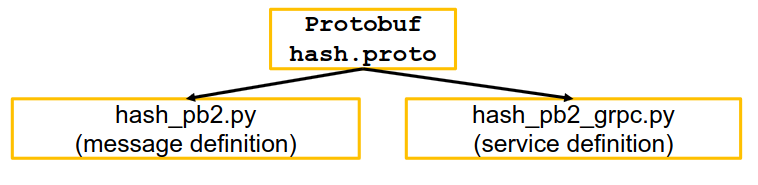
\includegraphics[width=9cm]{images/70.png}
    \end{center}
    Now that we have define all this, we can create our server using gRPC 
    \begin{tcolorbox}[violet]
        \textbf{Server creation using gRPC:}\\
        \begin{codeCenter}
        \begin{Ccode}
# hash_server.py
from hash_pb2_grpc import HashServicer // HashServicer is the ``server stub''
from hash_pb2 import HashRequest, HashResult
class HashServiceImpl(HashServicer):
    def GetHash(self, request:HashRequest, context):
        hash_result = HashResult()
        hash_result.result =str(hash(request.input))
        return hash_result
from concurrent import futures
request_thread_pool = futures.ThreadPoolExecutor(max_workers=10)
import grpc
server = grpc.server(request_thread_pool)

from hash_pb2_grpc import add_HashServicer_to_server
service_implementation = HashServiceImpl()
add_HashServicer_to_server(service_implementation, server)

server.add_insecure_port('[::]:50051')
server.start()
print("Hash server is running on port 50051 on local host...")
server.wait_for_termination()
        \end{Ccode}
        \end{codeCenter}
       \end{tcolorbox}
    Usually we should have done a TCP connection to communicate with the client. But gRPC channels abstract away communication, everything is built-in: streaming, retries, deadlines and cancellations.
    \begin{center}
        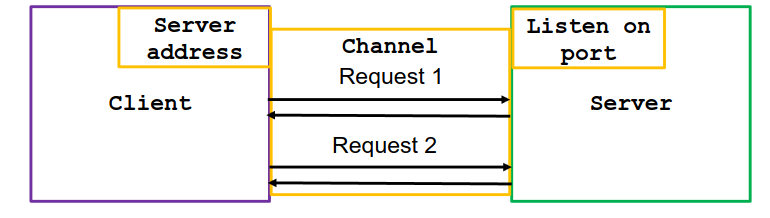
\includegraphics[width=9cm]{images/71.png}
    \end{center}
    \begin{tcolorbox}[gris]
    Now that we have our server, we have to create a client. We then need a stub as a substitute for server's services: it can be used instead of local procedure calls. We also need an address to where server is listening for requests (channel)

    \begin{codeCenter}
    \begin{Ccode}
# hash_client.py
import grpc
channel = grpc.insecure_channel('localhost:50051')

from hash_pb2_grpc import HashStub
stub = HashStub(channel)

from hash_pb2 import HashRequest
request = HashRequest(input="Hello world!")

from hash_pb2 import HashResult
response: HashResult = stub.GetHash(request)
print(f"Hash result for '{request.input}' is: {response.result}")
    \end{Ccode}
    \end{codeCenter}
    \end{tcolorbox}
    RPC and gRPC are everywhere:
    \begin{itemize}[left=10pt, label=\textbullet]
        \item In the industry, it is used by google cloud platform's services, LLM agents\ldots 
        \item In hardware, it is used to transports message to NIC:
            \begin{center}
                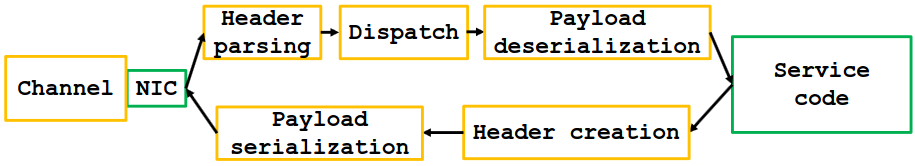
\includegraphics[width=11cm]{images/72.png} 
            \end{center}
    \end{itemize}
    \begin{image}{RPC layer takes 40-90\% of microservice time. \\

        Reduce CPU time on RPC overheads is an active area of research.}
        \begin{center}
        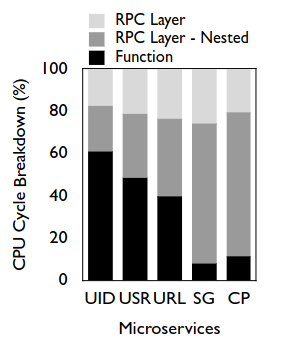
\includegraphics[width=4cm]{images/73.png}
        \end{center}
    \end{image}
